\documentclass[ignorenonframetext,]{beamer}
\usetheme{Warsaw}
\usecolortheme{sidebartab}
\usefonttheme{professionalfonts}


\usepackage{amssymb,amsmath}
\usepackage{ifxetex,ifluatex}
\usepackage{fixltx2e} % provides \textsubscript
\usepackage{lmodern}
\ifxetex
  \usepackage{fontspec,xltxtra,xunicode}
  \usepackage[cjk,hangul]{kotex}
  \defaultfontfeatures{Mapping=tex-text,Scale=MatchLowercase}
  \newcommand{\euro}{€}
\else
  \ifluatex
    \usepackage{fontspec}
    \defaultfontfeatures{Mapping=tex-text,Scale=MatchLowercase}
    \newcommand{\euro}{€}
  \else
    \usepackage[T1]{fontenc}
    \usepackage[utf8]{inputenc}
    \usepackage[cjk,hangul]{kotex}
      \fi
\fi
\IfFileExists{upquote.sty}{\usepackage{upquote}}{}
% use microtype if available
\IfFileExists{microtype.sty}{\usepackage{microtype}}{}
\usepackage{url}
\usepackage{letltxmacro}
\makeatletter
\def\maxwidth{\ifdim\Gin@nat@width>\linewidth\linewidth\else\Gin@nat@width\fi}
\def\maxheight{\ifdim\Gin@nat@height>\textheight0.8\textheight\else\Gin@nat@height\fi}
\makeatother
\AtBeginDocument{
  \LetLtxMacro\Oldincludegraphics\includegraphics
  \renewcommand{\includegraphics}[2][]{%
    \Oldincludegraphics[#1,width=\maxwidth,height=\maxheight,keepaspectratio]{#2}}
}

% Comment these out if you don't want a slide with just the
% part/section/subsection/subsubsection title:
\AtBeginPart{
  \let\insertpartnumber\relax
  \let\partname\relax
  \frame{\partpage}
}
\AtBeginSection{
  \let\insertsectionnumber\relax
  \let\sectionname\relax
  \frame{\sectionpage}
}
\AtBeginSubsection{
  \let\insertsubsectionnumber\relax
  \let\subsectionname\relax
  \frame{\subsectionpage}
}

\setlength{\parindent}{0pt}
\setlength{\parskip}{6pt plus 2pt minus 1pt}
\setlength{\emergencystretch}{3em}  % prevent overfull lines
\setcounter{secnumdepth}{0}

\title{6.4 서울 시장 선거 여론조사를 이용한 베이지언 추론}
\author{전희원}
\date{2014-06-24}

\begin{document}
\frame{\titlepage}

\begin{frame}{Background}

\begin{quote}
베이지언은 선거 예측에 많이 사용되어진 방법론이다. 가장 먼저 튜키 교수가
선거 예측에 베이지언을 사용했다고 알려져 있으며 이후 같은 방식으로
네이트 실바가 2008년에 미국 50개 주 중 49개 주, 그리고 2012년에는 50개
주 전체의 대선 결과를 정확히 예측하여 일대 파장을 일으켰다. 한국에서는
서울대학교 정치학과 박종희 교수가 지난 2013 대선 결과를 1\%의 에러로
예측한 사례가 있다.
\end{quote}

\end{frame}

\begin{frame}{Purpose}

\begin{itemize}
\itemsep1pt\parskip0pt\parsep0pt
\item
  박원순, 정몽준 두 후보들간의 지지율 차이 예측
\item
  빈도주의자들의 방법과 베이지언 방법의 결과 차이 분석
\item
  \texttt{6.4} 서울 시장 선거 실제 결과와 비교
\end{itemize}

\end{frame}

\begin{frame}{Data}

\begin{itemize}
\itemsep1pt\parskip0pt\parsep0pt
\item
  Data : 중앙선거관리위원회 \url{https://www.nesdc.go.kr}
\item
  Range : \texttt{2014-03-24} \textasciitilde{} \texttt{2014-05-28}
\item
  여론조사 수 : 31
\item
  조사기관 수 : 16
\item
  조사의뢰기관 수 : 21
\end{itemize}

\end{frame}

\begin{frame}{EDA}

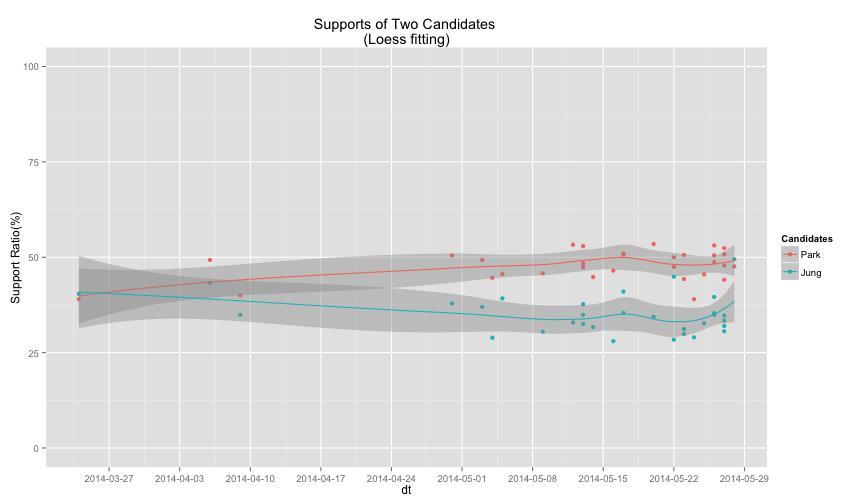
\includegraphics{./presentation_korean_files/figure-beamer/eda.png}

\end{frame}

\begin{frame}{Multinomial Likelihood with a Dirichlet Prior}

\begin{itemize}
\itemsep1pt\parskip0pt\parsep0pt
\item
  베이지안 : $P(\theta|X) \propto P(X|\theta)P(\theta)$
\item
  후보 지지자 수(j:정몽준, p :박원순, e :군소 후보/무응답)

  \begin{itemize}
  \itemsep1pt\parskip0pt\parsep0pt
  \item
    $n_j, n_p, n_e$
  \end{itemize}
\item
  Likelihood

  \begin{itemize}
  \itemsep1pt\parskip0pt\parsep0pt
  \item
    $X_j,X_p,X_e \sim Multinomial(n, \theta_{n_j}, \theta_{n_p}, \theta_{n_e})$
  \end{itemize}
\item
  Prior

  \begin{itemize}
  \itemsep1pt\parskip0pt\parsep0pt
  \item
    $\pi(\theta_j, \theta_p, \theta_e) \propto 1$
  \item
    $\theta_{n_j}, \theta_{n_p}, \theta_{n_e} \sim Dirichlet(1,1,1)$
  \end{itemize}
\item
  Posterior

  \begin{itemize}
  \itemsep1pt\parskip0pt\parsep0pt
  \item
    $\theta_{n_j}, \theta_{n_p}, \theta_{n_e}|n_j,n_p,n_e \sim Dirichlet(n_j + 1, n_p + 1, n_e + 1)$
  \end{itemize}
\end{itemize}

\end{frame}

\begin{frame}{Steps}

\begin{enumerate}
\def\labelenumi{\arabic{enumi}.}
\itemsep1pt\parskip0pt\parsep0pt
\item
  무정보 사전 확률 셋업
\item
  새로운 여론 조사 결과가 나올때마다 이전 사전확률을 기반으로 사후확률을
  계산\ldots{}(반복)
\item
  몬테칼로 시뮬레이션을 수행해 각 파라메터 분포 생성(10,000 samples).
\item
  파라메터 분포를 기반으로 $\theta_p - \theta_j$ 계산 지지율 차이 분포
  생성
\end{enumerate}

\end{frame}

\begin{frame}{Mean of Posterior}

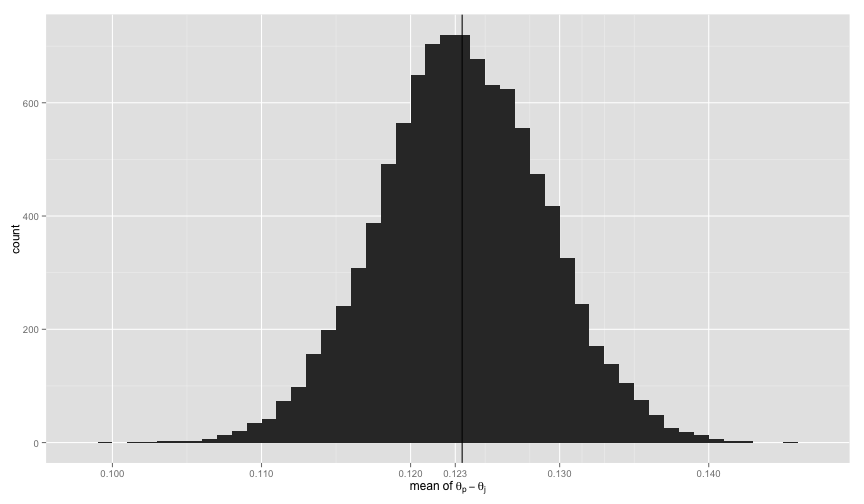
\includegraphics{./presentation_korean_files/figure-beamer/mc.png}

\end{frame}

\begin{frame}{Comparison between Frequentist and Bayesian}

\begin{itemize}
\itemsep1pt\parskip0pt\parsep0pt
\item
  전통적 모비율 차이 추정식(Frequentist's)

  \begin{itemize}
  \itemsep1pt\parskip0pt\parsep0pt
  \item
    $\hat{p_p} - \hat{p_j} \pm \frac{Z_{a/2}}{\sqrt{N}}\sqrt{\frac{N - n}{N}}\sqrt{\hat{p_p}(1 - \hat{p_p}) + \hat{p_j}(1 - \hat{p_j}) + 2\hat{p_p}\hat{p_j}}$
  \end{itemize}
\end{itemize}

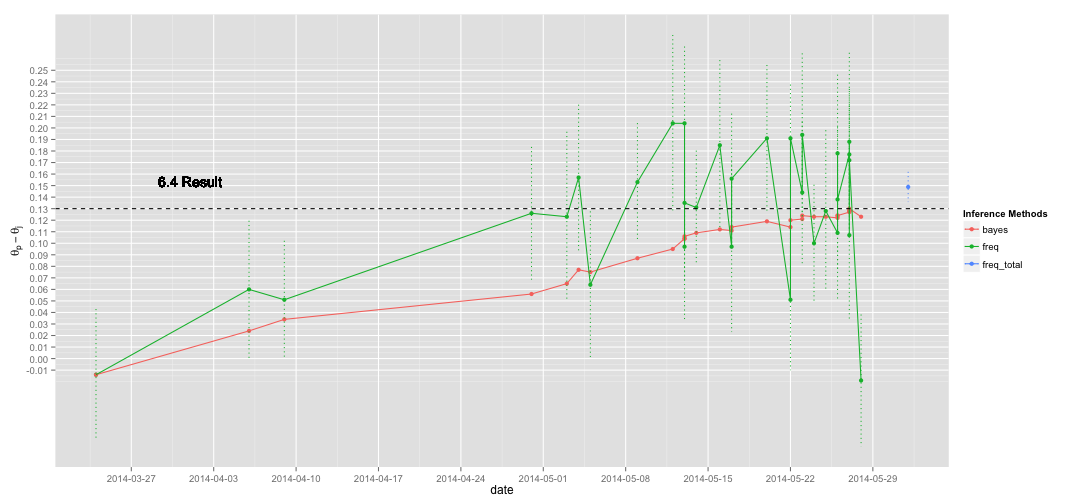
\includegraphics{./presentation_korean_files/figure-beamer/comp.png}

\end{frame}

\begin{frame}{Conclusion}

\begin{itemize}
\itemsep1pt\parskip0pt\parsep0pt
\item
  전통적인 여론조사 기반 예측은 개별 건에 대한 예측값만 도출하나
  베이지언은 여러 데이터를 기반으로 시계열적인 특징을 부여해 예측할 수
  있다.
\item
  베이지언은 꽤 정확한 결과를 도출해 준다(0.0066 error).
\item
  \texttt{2014-05-28}일자의 잘못된 여론조사 결과를 제외할 경우 실제
  결과인 \texttt{13\%} 차이를 정확히 예측한다.
\end{itemize}

\end{frame}

\begin{frame}{Q \& A}

\begin{itemize}
\itemsep1pt\parskip0pt\parsep0pt
\item
  References

  \begin{itemize}
  \itemsep1pt\parskip0pt\parsep0pt
  \item
    Gelman, et. al. Bayesian Data Analysis 3nd (2013, p.~69)
  \item
    Andrew D. Martin, Kevin M. Quinn, Jong Hee Park (2011). MCMCpack:
    Markov Chain Monte Carlo in R. Journal of Statistical Software.
    42(9): 1-21. URL \url{http://www.jstatsoft.org/v42/i09/}.
  \end{itemize}
\item
  Code and Data

  \begin{itemize}
  \itemsep1pt\parskip0pt\parsep0pt
  \item
    \url{https://github.com/haven-jeon/2014_Seoul_Mayoral_Election_Analysis}
  \end{itemize}
\end{itemize}

\end{frame}

\end{document}
